\subsection{Choix Techniques}

\begin{frame}{Choix du langage de programmation}
	\begin{block}{C++}
  	\begin{itemize}
    	\item rapidité d'éxecution
    	\item langage à objets
    	\item connaissance du langage
    	\item langage très répandu
  	\end{itemize}
	\end{block}
\end{frame}

\begin{frame}{Utilisation d'un gestionnaire de version}
	\begin{block}{git - the stupid content tracker}
  	\begin{itemize}
    	\item sauvegarde
    	\item partage
    	\item mise en commun
  	\end{itemize}
	\end{block}
\end{frame}

\subsection{Structures}
\begin{frame}{Représentation du problème de flot maximum}
	\begin{block}{Réseau de transport}
  	\begin{itemize}
    	\item Graphe orienté pondéré
    	\item une source
    	\item un puits
  	\end{itemize}
	\end{block}
	\begin{block}{Graphe d'écarts}
  	\begin{itemize}
    	\item Graphe orienté pondéré
  	\end{itemize}
	\end{block}
\end{frame}


\begin{frame}{Représentation du problème de flot maximum}
	\begin{block}{Graphe de couches}
  	\begin{itemize}
    	\item Graphe orienté pondéré
  	  \item Représenation des couches par un tableau de listes de sommets.
  	\end{itemize}
	\end{block}
\end{frame}

\begin{frame}{Diagramme de classes}
	\begin{figure}
	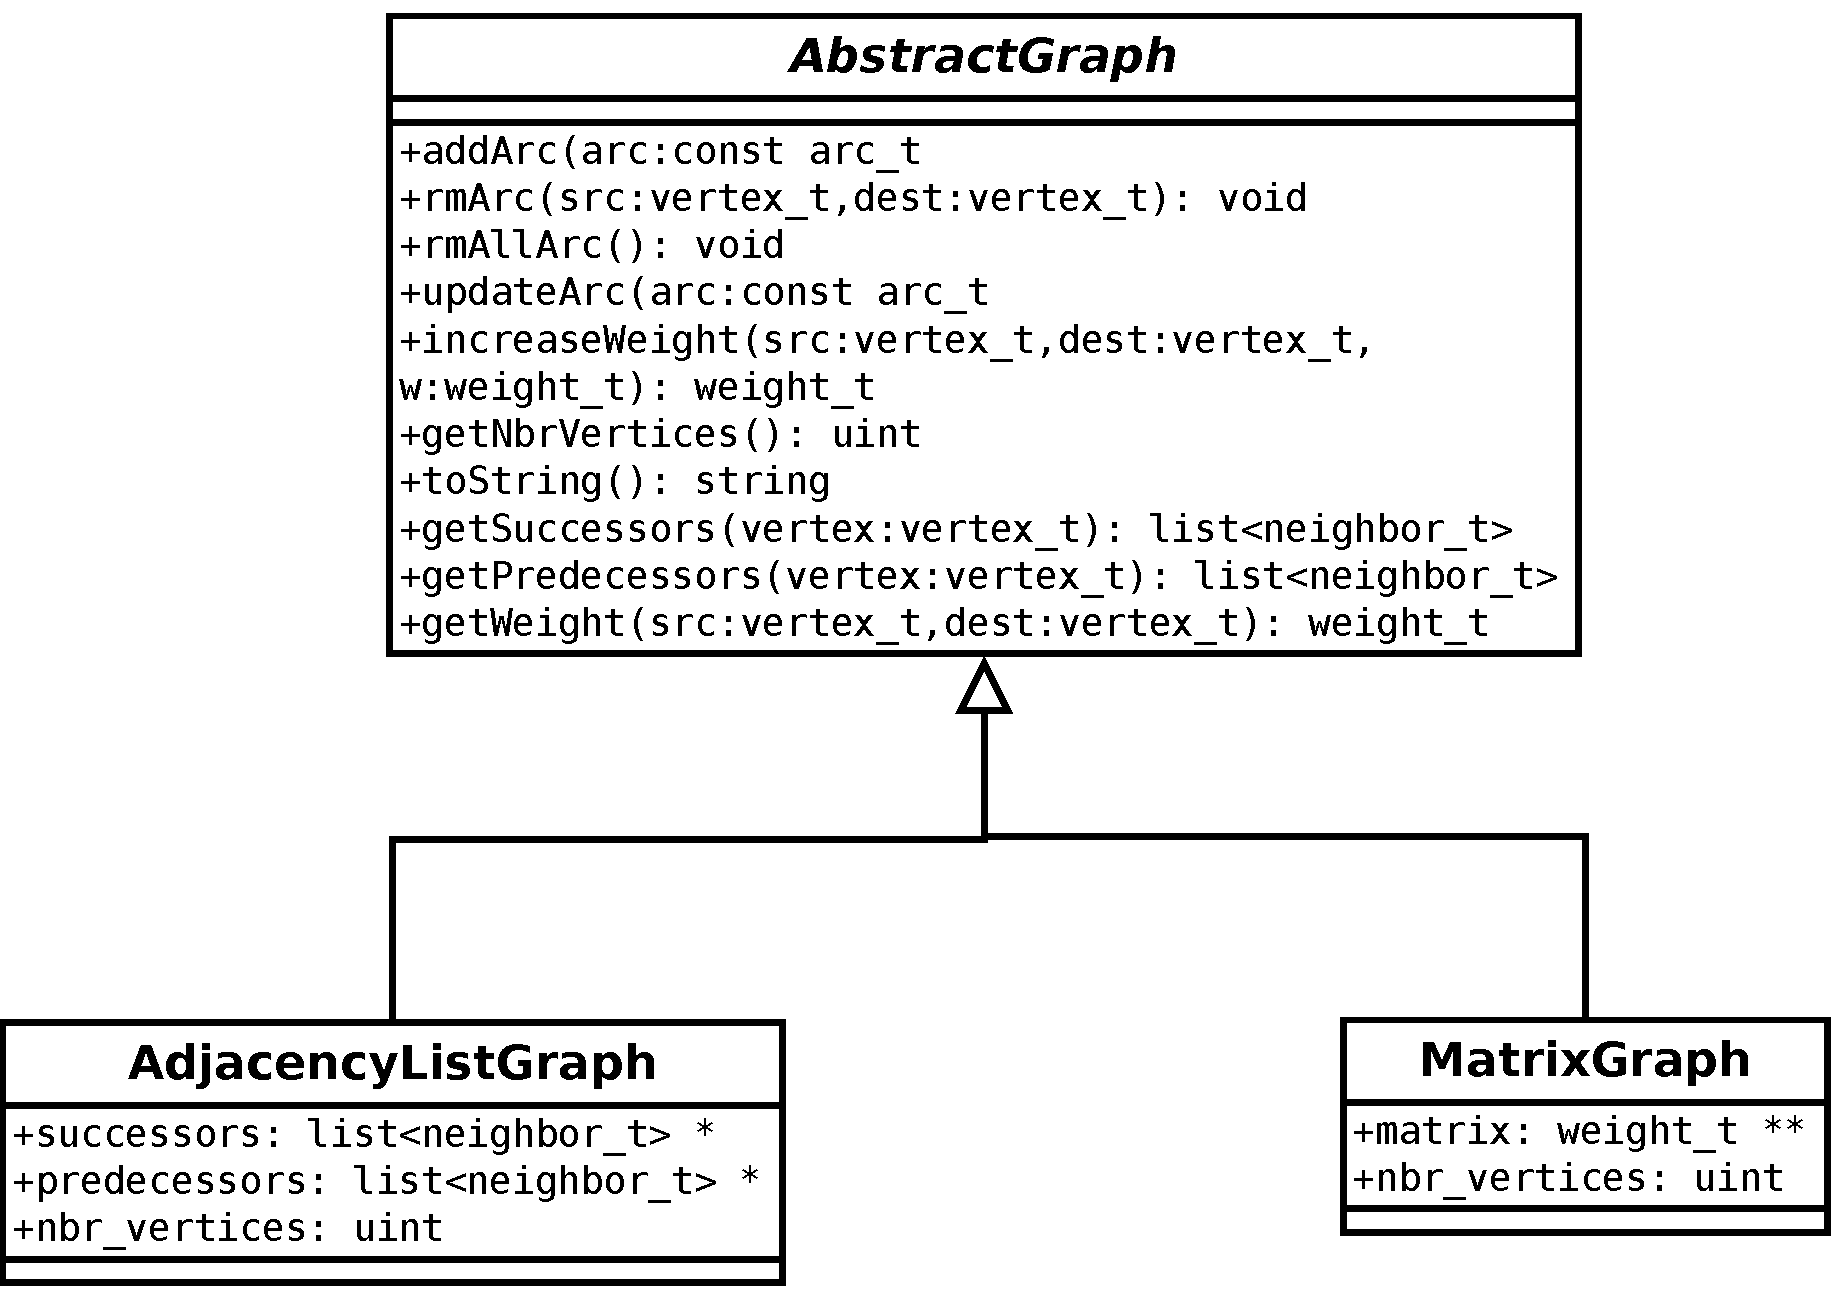
\includegraphics[width=0.8\textwidth]{img/diag_class.pdf}
	\end{figure}
	% Classe abstraite pour s'abstraire dans les algos des structures de données
\end{frame}

\subsection{Mise en oeuvre des algorithmes}

\begin{frame}{Edmonds-Karp}
	\begin{block}{Recherche du plus court chemin en nombre d'arcs}
  	Parcours en largeur
  	\begin{itemize}
    	\item Graphes en listes d'adjacences : O(n+m)
  	  \item Graphes en matrice d'adjacences : O($n^2$)
  	\end{itemize}
  \end{block}
  \begin{block}{Mise à jour du graphe d'écart}
  	Parcours du chemin \\
  	Décrementation du poids de chaque arc u,v du chemin \\
  	Incrémentation du poids de chaque arc v,u \\
  	\begin{itemize}
    	\item Graphes en listes d'adjacences : O(n+m)
  	  \item Graphes en matrice d'adjacences : O(n)
  	\end{itemize}
  \end{block}
\end{frame}

\begin{frame}{Dinic}
	\begin{block}{Génération du graphe de couches}
  	Parcours en largeur + stockage d'une liste de parents par sommets
  \end{block}
  \begin{block}{Calcul du flot bloquant}
  	Parcours en largeur + stockage d'une liste de parents par sommets
  	\begin{itemize}
    	\item Graphes en listes d'adjacences : O(nm)
  	  \item Graphes en matrice d'adjacences : O($n^2$m)
  	\end{itemize}
  \end{block}
	\begin{block}{Mise à jour du graphe d'écart}
  	Pour chaque arcs du flot bloquant \\
  	Décrementation du poids de chaque arc u,v du chemin \\
  	Incrémentation du poids de chaque arc v,u \\
  	\begin{itemize}
    	\item Graphes en listes d'adjacences : O($m^2$)
  	  \item Graphes en matrice d'adjacences : O($n^2$)
  	\end{itemize}
  \end{block}
\end{frame}

\begin{frame}{Génération de réseaux de transport aléatoires}
	\begin{block}{Deux stratégies}
  	\begin{itemize}
  		\item Tirage aléatoire de deux sommets
  		\item Génération de tous les arcs possibles et tirage d'un arc
  	\end{itemize}
	\end{block}
\end{frame}